% Source: tex/chapters/ch05/08_テストプロセス.tex
\subsection{テストプロセス}
テスト技法や測度は、定義されたテストプロセスに組み込まれて初めて実務で機能する。テストプロセスは、組織レベル、管理レベル、動的テストレベルの多層構造で考えられる。組織レベルでは方針や戦略を作る。管理レベルでは計画、監視、制御、完了を扱う。動的テストレベルでは設計、実装、環境構築、実行、インシデント報告を扱う。

\begin{figure}[htbp]
\centering
\IfFileExists{assets/fig-ch05-12.png}{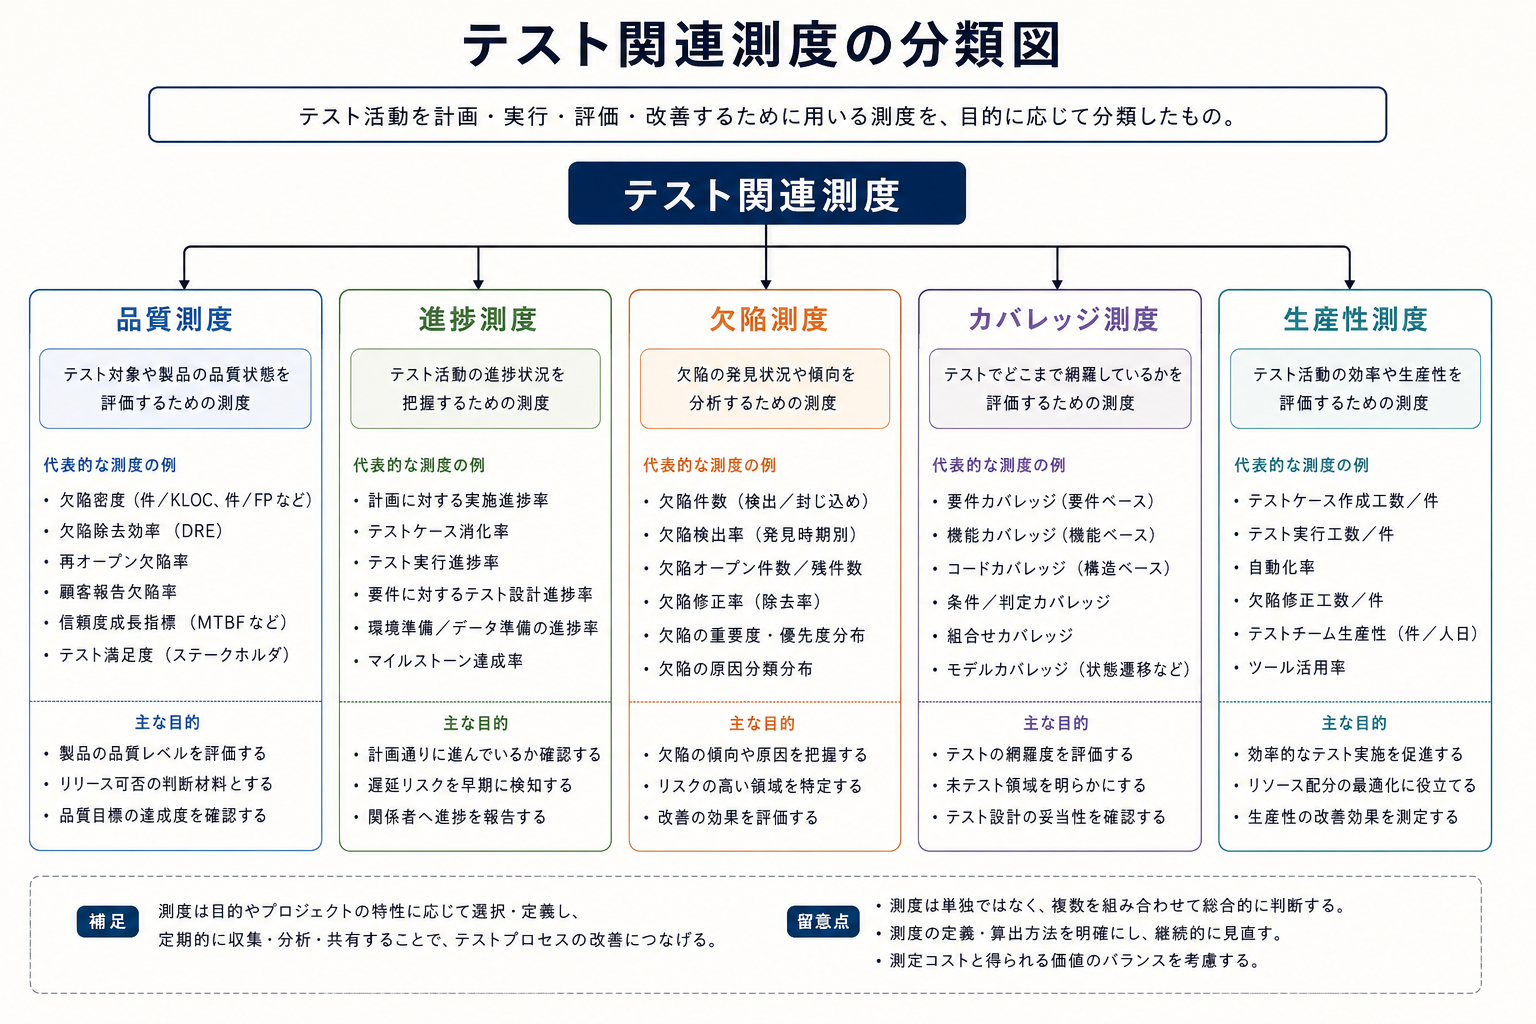
\includegraphics[width=0.96\linewidth]{assets/fig-ch05-12.png}}{\fbox{\parbox[c][48mm][c]{0.9\linewidth}{\centering 画像生成待ち\\テストプロセスの多層図}}}
\caption{テストプロセスの多層図}
\label{fig:ch05-12}
\end{figure}
